\documentclass{tnreport}
%\documentclass[stage2a]{tnreport} % If you are in 2nd year
%\documentclass[confidential]{tnreport} % If you are writing confidential report

\def\reportTitle{
	Implémentation d’un service de liste de confiance globale basé sur la blockchain
	%Implémentation d’une Global Trust Service Status List basé sur la blockchain
	%Implémentation d'une liste globale des services de confiance basée sur la blockchain
	%Implémentation d'une liste mondiale de confiance basée sur la blockchain
} % Titre du mémoire
\def\reportLongTitle{
	Implémentation d’un service de liste de confiance globale basé sur la blockchain
	%Implémentation d’un service de trust list global basé sur la blockchain
	%Implémentation d'un service de liste globale des services de confiance basé sur la blockchain
} % Titre plus long du mémoire

\def\reportAuthor{Yoann Raucoules}
\def\reportAuthorEmail{\email{yoann.raucoules@telecomnancy.eu}} % Courriel de l'élève

\def\reportAuthorAddress{6, rue du général Frère} % Adresse de l'élève
\def\reportAuthorCity{57070, METZ} % Adresse (cont.) de l'élève
\def\reportAuthorPhone{+33 (0)6 77 48 04 38} % Téléphone de l'élève 

\def\reportIndustrialSupervisor{Vincent Bouckaert} % Prénom Nom de l'encadrant industriel
\def\reportAcademicSupervisor{Olivier Festor} % Prénom Nom de l'encadrant académique

\def\reportCompany{ARHS Spikeseed} % Nom de l'entreprise d'accueil
\def\reportCompanyAddress{2B, rue Nicolas Bové}  % Adresse de l'entreprise
\def\reportCompanyCity{1253, LUXEMBOURG} % Adresse (cont.) de l'entreprise
\def\reportCompanyPhone{+352 26 11 02 1} % Téléphone de l'entreprise
\def\reportCompanyLogoPath{figures/logo-arhs-spikeseed} % Logo de l'entreprise -- comment this definition to remove company logo

\def\place{Luxembourg} % Ville pour la signature pour l'engagement anti-plagiat
\def\date{\today} % Date pour la signature de l'engagement anti-plagiat

\usepackage{textgreek}

\begin{document}
  
\maketitle
\pagenumbering{roman}

\insertAntiPlagiarismAgreement{Raucoules, Yoann}{1205028998}

\cleardoublepage

\makesecondtitle

\section*{Remerciements}
\addcontentsline{toc}{chapter}{Remerciements}

{\em
``Night gathers, and now my watch begins. \\
It shall not end until my death.

I shall take no wife, hold no lands, father no children. \\
I shall wear no crowns and win no glory. \\
I shall live and die at my post.

I am the sword in the darkness. \\
I am the watcher on the walls. \\
I am the shield that guards the realms of men.

I pledge my life and honor to the Night's Watch, \\
for this night and all the nights to come.''
}

\hspace{4cm} -- The Night's Watch oath


\cleardoublepage

\section*{Avant-propos}
\addcontentsline{toc}{chapter}{Avant-propos}

Ce mémoire résulte d'un stage de fin d'études qui s'est déroulé du 3 avril 2017 au 30 septembre 2017 au sein de l'entreprise Ar{\texteta}s Spikeseed située au Luxembourg. Ce stage vient clôturer et valider la formation d'ingénieur du numérique de l'école TELECOM Nancy que j'ai débuté en septembre 2014. Cette formation qui s'est étendue sur une période de trois ans m'a permis d'acquérir de nombreuses compétences dans les domaines de l'informatique, des mathématiques, du management, de la gestion de projet, de la communication, de l'économie, du droit et des langues. J'ai choisi de me spécialiser en Ingénierie Logicielle au cours du cursus de par ma passion pour la programmation et l'architecture logicielle depuis que j'ai découvert l'informatique lors de mon stage de découverte professionnelle réalisé en classe de troisième.

Au cours de ce stage de fin d'études, j'ai eu le plaisir de travailler sur une technologie à laquelle je m'intéresse depuis deux ans, la blockchain. Dans le cadre d'un projet proposé par la Commission Européenne, nommé FutureTrust, j'ai pu concevoir et implémenter un service de trust list global basé sur la blockchain. Mes tâches ont été de me familiariser avec les principes de la blockchain et les concepts de cryptographie appliquée afin de les mettre en application dans le projet, d'effectuer une analyse des solutions de blockchain existantes afin de réaliser des choix d'implémentation, de concevoir l'architecture du service de liste de confiance globale, d'implémenter la solution conçue et de documenter tous les aspects techniques et fonctionnels de la solution implémentée.

Dans ce mémoire est présenté le résultat du stage de fin d'études et est mis en avant l'utilisation de la blockchain dans le cadre d'un projet de confiance numérique d'échelle mondiale. L'intérêt de ce document est dans un premier temps d'expliquer les tâches réalisées au cours du stage et dans un second temps de montrer qu'il est possible d'élargir le champ d'application de la technologie blockchain et des différents aspects qui la composent.
%de montrer que le champ d'application de la technologie blockchain peut être encore élargi.

\cleardoublepage

\renewcommand{\baselinestretch}{0.5}\normalsize
\tableofcontents
\renewcommand{\baselinestretch}{1.0}\normalsize
\cleardoublepage

\pagenumbering{arabic}
\setcounter{page}{1}

\chapter{Introduction}

La technologie blockchain s'est popularisée ces dernières années grâce à l'expansion de la crypto-monnaie\footnote{La crypto-monnaie aussi appelée monnaie cryptographique est une monnaie électronique basé sur les principes de la cryptographie.} Bitcoin\footnote{Bitcoin est une crypto-monnaie et un système de paiement pair-à-pair}~\cite{Bitcoin} à travers le monde. 
En effet, cette technologie a bouleversé aussi bien le monde de l'informatique que le monde de la finance. 
L'investissement autour de la blockchain a mené à un engouement général pour ce concept. 
Le Bitcoin a réussi à remettre en cause des acteurs majeurs de notre société tels que les banques ou les géants du Web, en sécurisant des échanges d'actifs sans organe central de contrôle. 
La révolution qu'il a engendré amène aujourd'hui les gouvernements et autres organisations publiques à réfléchir sur la régulation de la technologie et des crypto-monnaies naissantes.
Depuis son lancement en 2009, la blockchain n'a cessé d'évoluer et d'étendre son champ d'application.
Bien qu'à l'origine elle a été conçue pour le transfert de crypto-monnaie, les avantages qu'elle apporte permettent d'imaginer de multiples cas d'utilisation qui dépassent son cadre initial d'échanges d'actifs.
À l'heure où l'ubérisation\footnote{L'ubérisation est un phénomène économique désignant l'utilisation de services permettant aux professionnels et aux clients de se mettre en contact direct grâce à l'utilisation des nouvelles technologies} de notre société est en marche, la technologie blockchain amène une approche nouvelle 
qui permet de se détacher de toute organe central ou tierce partie. 
La blockchain ira-t-elle jusqu'à ubériser\footnote{Ubériser est le verbe issu du substantif ubériser} Uber\footnote{Uber est l'entreprise qui déclencha ce qu'on appelle l'ubérisation} ?

\section{Présentation de la technologie blockchain}

Une blockchain est basée sur l'échange d'actifs numériques, réalisé grâce à des transactions signées, et agit comme un registre publique distribué où toutes les transactions y sont répertoriées. Elle repose sur des principes de cryptographie afin d'assurer l'intégrité de ces transactions et sur un protocole décentralisé, dit {\em peer-to-peer}, qui permet à la blockchain d'avoir une disponibilité maximale et d'établir un consensus entre les participants du réseau afin de protéger contre les falsifications.

Si cette technologie connaît un tel succès c'est parce qu'elle apporte de nombreux avantages : 
\begin{itemize}
	\item la décentralisation, qui signifie que son architecture ne repose pas sur une entité centrale et permet d'enregistrer des données dans un réseau distribué; 
	\item la transparence, puisque l'état des données conservées est consultable publiquement par tout le monde; 
	\item l'autonomie, puisqu'elle est basée sur un consensus dans lequel chaque partie prenante peut transférer des données de manière sécurisée et autonome;
	\item l'immutabilité, en effet toute transaction est persistée définitivement et donc ne peut être effacée;
	\item l'anonymat, car toute personne est anonyme dans le sens où elle n'est pas désignée par son identité mais uniquement par une clé publique\footnote{Une clé publique est un encodage rendu public dans le cadre d'un échange d'informations utilisant le principe de la cryptographie asymétrique}.
\end{itemize}
%la décentralisation, qui signifie que son architecture ne repose pas sur une entité centrale et permet d'enregistrer des données dans un réseau distribué; 
%la transparence, puisque l'état des données conservées est consultable publiquement par tout le monde; 
%l'autonomie, puisqu'elle est basée sur un consensus dans lequel chaque partie prenante peut transférer des données de manière sécurisée et autonome;
%l'immutabilité, en effet toute transaction est persistée définitivement et donc ne peut être effacée;
%l'anonymat, car toute personne est anonyme dans le sens où elle n'est pas désignée par son identité mais uniquement par une clé publique.

\section{Définition du cadre et des objectifs du stage}

Dans ce contexte, un stage ingénieur a été réalisé sur une période de 6 mois au sein de la société Arηs Spikeseed située au Luxembourg. 
Le stage a été réalisé dans les locaux de l'entreprise, la langue officielle du projet pour les communications avec les autres membres du consortium (mails, documents, conférence téléphonique) est l’anglais, il en est de même pour la langue utilisée au sein de l'équipe puisque c'est une équipe multinationale. Les documents produits, et présentés dans ce mémoire, ont donc été rédigés en anglais.
Ce stage de fin d'études a pour objectif d'intégrer la technologie blockchain au sein d'un processus de gestion de listes de services de confiance dans le cadre d'un règlement européen. 
La finalité est d'utiliser cette technologie afin de conserver des données publiques relatives à la confiance électronique de manière sécurisée et décentralisée en utilisant une blockchain en tant que registre.
Cela a pour but d'assurer la disponibilité et l'intégrité des informations, puisque les données sont distribuées à travers les nœuds du réseau et sécurisées à l'aide de transactions signées et vérifiées par une preuve mathématique. 

\section{Mise en exergue du plan}

\textbf{ÉDIT EN FONCTION DU PLAN DÉFINITIF}

\textit{
Ce mémoire vise à montrer que le champ d'application de la technologie blockchain dépasse son cadre initial et que son utilisation permet de pallier aux problèmes d'architecture et de sécurité des modèles actuels. 
Dans un premier temps, le contexte du projet sera défini, puis la problématique, qui détaillera les limites des architectures actuelles, sera exposée. 
Ensuite, sera établit un état de l'art afin de comparer les outils existants et de justifier les choix opérés durant le stage. 
Après cela, la réalisation du projet sera développée en expliquant: 
le choix de l'architecture mise en place; 
l'avantage de persister des données dans un système de fichiers décentralisé; 
l'intérêt de gérer l'authentification des utilisateurs par la mise en place d'un consensus; 
l'implémentation d'un système de contrôle de versions et d'un moteur de recherche sur des données stockées dans un réseau décentralisé et distribué. 
Enfin, les résultats obtenus et les perspectives du projet seront détaillés.
}

\chapter{Présentation du contexte}

\section{L'entreprise Ar{\texteta}s Spikeseed}

Ar{\texteta}s Spikeseed est une entité du groupe Ar{\texteta}s qui est une entreprise de services du numérique (ESN) fondée en 2003 par Jourdan Serderidis. 
Le groupe est divisé en sociétés réparties au Luxembourg, en Belgique, en Grèce et depuis cette année en Italie. Le groupe Ar{\texteta}s possèdent cinq axes de compétences qui sont présentés dans la Figure~\ref{fig:arhs-core-services}.

\begin{figure}[h]
	\centering
	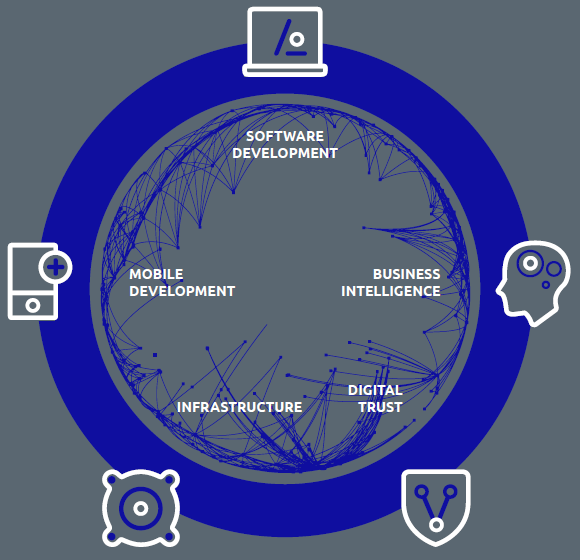
\includegraphics{figures/arhs-core-services}
	\caption{Axes de compétences du groupe Ar{\texteta}s \cite{annual-report}}
	\label{fig:arhs-core-services}
\end{figure}

Comme toutes les autres entités du groupe, Ar{\texteta}s Spikeseed vise à délivrer des solutions numériques complexes. Elle a la particularité de réaliser principalement des projets de recherche et développement en s'appuyant sur les pratiques agiles et des technologies de pointe. 
De plus, Ar{\texteta}s Spikeseed est compétente afin de mettre en œuvre: 
des solutions liées à la confiance numérique; 
des systèmes engageant des masses de données grâce à des technologies innovantes et efficaces comme le Web sémantique ou la Business intelligence; 
des applications destinées aux mobiles et aux objets connectés.

\section{Contexte du projet}

Dans le cadre d'un règlement de l'Union Européenne (UE) sur l'identification électronique (eID) et les services de confiance pour les transactions électroniques sécurisées au sein de l'UE (eIDAS), la Commission Européenne (CE) a émis un appel à projet qui a pour visée de supporter la mise en œuvre technique de ce règlement européen. 
Ce projet de recherche et développement appelé FutureTrust rassemble un consortium de seize partenaires, dont Ar{\texteta}s Spikeseed, engagé dans la réalisation et la mise en application du règlement européen. 
Le projet FutureTrust répondra au besoin de solutions globales et interopérables, en fournissant des logiciels libres qui faciliteront l'utilisation de l'identification et de la signature électronique. 
Il vise à étendre l'infrastructure de la liste européenne de services de confiance existante vers une liste mondiale des services de confiance, nommée Global Trust Service Status List (gTSL), à développer un service de validation ainsi qu'un service d'archivage pour les signatures et les sceaux électroniques, et à fournir des composants pour les certificats qualifiés et pour la création de signatures et de sceaux dans un environnement mobile.

Ce stage de fin d'études a porté sur l'intégration la technologie blockchain dans le cadre du projet FutureTrust et plus particulièrement sur son intégration dans le module de gTSL. Les autres modules du projet ne seront pas détaillés dans ce document. 

\chapter{Présentation détaillée de la problématique}

Les architectures logicielles évoluent en suivant les innovations technologiques. Aujourd'hui, le domaine de la recherche apporte des nouvelles technologies ou des améliorations aux concepts existants à une vitesse exponentielle, si bien que 
le temps de réalisation d'un projet le rend obsolète lors de sa livraison.
%lorsqu'un projet est livré au client celui-ci est déjà presque obsolète. 
Le meilleur exemple de ce phénomène est le framework Angular, initié par Google, qui est passé de la version 2 à la version 5 en moins d'une année. C'est la réalité actuelle de l'univers technologique poussé par l'innovation, un monde où les acteurs doivent s'adapter en permanence aux changements. La technologie blockchain s'inscrit dans ces innovations récentes issues de la recherche. Elle amène une nouvelle vision d'un Internet décentralisé sans organe central de contrôle, qui va probablement révolutionner la conception des systèmes d'information dans les prochaines années. Dans ce contexte, l'utilisation de la blockchain a été proposée dans le cadre du projet FutureTrust.

\section{Description du service de trust list global}

%\subsubsection{Business Purpose}
%\section{Détail }

{\em
\begin{itemize}
	\item Détail du sujet
	\item (design document 4. Requirements)
	\item (schéma page 15 ETSI 119 612: Structure d'une TSL)
\end{itemize}
}

Les États membres de l'UE et d'autres pays européens maintiennent généralement des listes d'autorités de certification et d'autres fournisseurs de services de confiance, désignés Trust Service Providers (TSP), dans un ou plusieurs registres à l'échelle nationale.
La liste de confiance des États membres de l'UE comprend des informations relatives aux TSPs qualifiés qui sont supervisés par l'État membre compétent, ainsi que des informations relatives aux services de confiance, désignés Trust Services (TS), qu'ils fournissent, conformément aux dispositions prévues par le règlement eIDAS.
Les listes de confiance sont des éléments essentiels dans la mise en place de la confiance numérique pour les opérateurs du marché électronique, en permettant aux utilisateurs de déterminer le statut qualifié des TSPs et de leurs TSs. En vertu du règlement eIDAS, les listes nationales de confiance ont un effet constitutif.
En d'autres termes, un fournisseur ou un service ne sera qualifié que s'il apparaît dans les listes de confiance. Par conséquent, les utilisateurs (citoyens, entreprises ou administrations publiques) bénéficieront de l'effet juridique associé à un service de confiance qualifié donné uniquement si ce dernier est répertorié (comme qualifié) dans les listes de confiance.	
Les États membres peuvent inclure dans les listes de confiance des informations sur les fournisseurs de services de confiance non qualifiés et sur d'autres services de confiance définis au niveau national.

La structure d'une liste de confiance est présentée dans la Figure~\ref{fig:tsl-scheme}.

\begin{figure}[h]
	\centering
	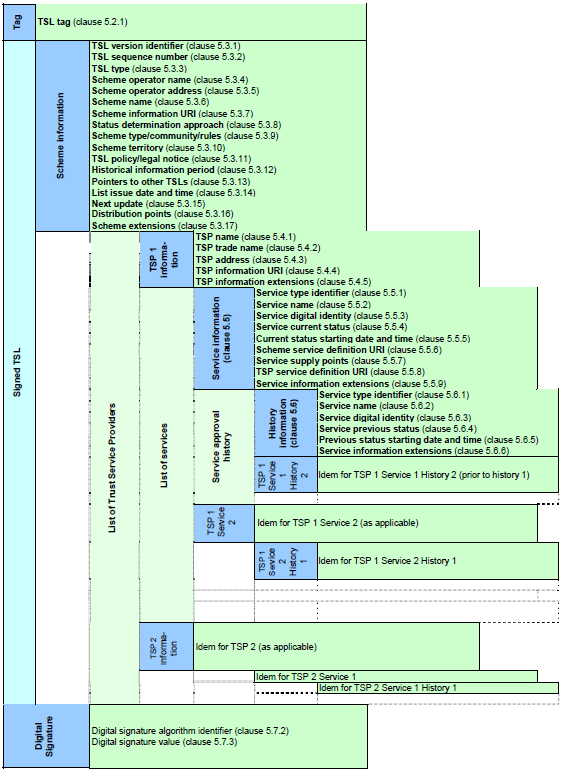
\includegraphics{figures/gTSL-TSLScheme}
	\caption{gTSL – Structure d'une liste de confiance}
	\label{fig:tsl-scheme}
\end{figure}

\clearpage

%\subsection{Stakeholder Requirements}
\subsection{Besoins générales}

%\subsubsection{Business Purpose}
\subsubsection{Intérêt du projet}

L'intérêt d'un service de 
%liste mondiale des services de confiance 
gTSL 
est de favoriser l'établissement de relations de confiance entre les opérateurs du marché en Europe et au-delà. À ce titre, elle étend le schéma actuel de la liste des services de confiance, dont la portée est uniquement européenne. Cette liste a pour but de répertorier les TSPs, ayant un statut qualifié ou non. On entend par statut qualifié que le TSP ait été accrédité par un organisme compétent au sein de l’État membre dans lequel le TSP est déclaré. Le service permet aux utilisateurs finaux de vérifier le statut de ces TSPs et d'accéder à l'ensemble des informations concernant les services de confiance.

%The business purpose of the Global Trust Status List Service specified in the present document is to foster the building of trust relationships between market operators across Europe, and beyond. As such, it extends the current Trust Status List scheme which indicates whether Trust Service Providers have a qualified status or not.

%\subsubsection{Stakeholders}
\subsubsection{Parties prenantes}

Les acteurs principaux de la 
%liste mondiale des services de confiance
gTSL
sont:
\begin{itemize}
	\item les États membres de l'UE, qui doivent établir, maintenir et publier les listes de confiance, incluant les informations relatives aux TSPs de services déclarés au sein de leur État;
	\item les fournisseurs de services de confiance, qui sont destinés à s'appuyer sur le service de gTSL dans lequel sont publiés leur statut qualifié et leurs informations publiques;
	\item les opérateurs de liste de confiance ne faisant pas partie d'un État membre de l'UE, qui souhaitent intégrer leur liste dans la gTSL;
	\item les citoyens de l'UE et non UE, qui sont destinés à utiliser le service afin d'accéder aux statuts et aux informations des différents TSPs répertoriés dans la gTSL.
\end{itemize}

%\subsubsection{Goal and Objective}
\subsubsection{Objectif du projet}

L'objectif principal de la gTSL est de gérer et de fournir les informations relatives aux TSPs qualifiés au sein de l'Union Européenne et au-delà, en étendant le modèle actuel de la liste européenne de services de confiance. De plus, cette réorganisation de l'architecture vise à gérer la gTSL de manière décentralisée dans le but d'en améliorer sa résilience ainsi que sa gestion.

\subsection{Besoins du système}

\subsubsection{Objectif du système}

En s'appuyant sur la norme de listes de confiance définie dans ETSI TS 119 612~\cite{ETSITS119612}, la gTSL vise à résoudre les imperfections actuelles du schéma de liste de confiance lorsqu'il est considéré dans un contexte globalisé. 
À l'heure actuelle, la Commission européenne publie une liste signée de pointeurs, nommée European List of the Lists (LoTL), dans laquelle chaque pointeur désigne un point de distribution pour une liste nationale de TSPs. 
Ces listes nationales contiennent des informations sur les TSPs qualifiés et non qualifiés ainsi que sur les services qualifiés ou non qualifiés qu'ils proposent.
Avec le modèle actuel, les modifications apportées au contenu d'une liste nationale induisent la nécessité de republier toute la liste nationale. De plus, toutes modifications apportées sur l'URL\footnote{Une URL (acronyme anglais de Uniform Resource Locator) est couramment appelé adresse web.} à laquelle la liste est distribuée ou sur le certificat utilisé pour signer la liste, induisent la nécessité de republier à la fois la liste nationale et la liste européenne.
Le caractère centralisé du système de distribution des listes de confiance actuel contient des potentiels problèmes qui doivent être résolus dans le cadre de la globalisation des listes de services de confiance:
\begin{itemize}
	\item les lites des États membres sont uniquement récupérable en basant sur la LoTL, le schéma actuel est donc sujet à un point individuel de défaillance\footnote{Un point individuel de défaillance (single point of failure ou SPOF en anglais) est un point d'un système informatique dont le reste du système est dépendant et dont une panne entraîne l'arrêt complet du système};
	\item des problèmes de performance et de latence peuvent être rencontrés puisqu'il est nécessaire de télécharger et valider l'ensemble des informations qui sont réparties sur différents points de distribution;
	\item l'architecture actuelle nécessite que l'ensemble des nœuds de distribution des États membres soit actifs car dans le cas contraire les informations des TSPs des États membres dont le nœud n'est pas actif ne sont plus disponibles;
	\item le schéma actuel ne conserve pas l'historique des modifications, c'est-à-dire qu'une nouvelle publication d'une liste remplace totalement la précédente, ce qui ne permet pas de conserver une trace des modifications mises en œuvre entre les versions.
\end{itemize}

\subsubsection{Portée du système}

La portée de la gTSL concerne la définition de services de confiance qualifiés et de fournisseurs de services de confiance.
À ce titre, elle fournira les fonctions nécessaires à la création, à la mise à jour et à la distribution des fournisseurs de services de confiance et des informations concernant leurs services de confiance.

\subsubsection{Présentation du système}

Afin d'atteindre ses objectifs, le gTSL s'appuiera sur deux principaux composants open source:
\begin{itemize}
	\item Global Trust Service Lifecycle Manager\footnote{en français, Gestionnaire du cycle de vie}
	\item Global Trust Service Responder\footnote{en français, Répondeur (dans le sens où il répond aux requêtes des utilisateurs)}
\end{itemize}
De plus, la gTSL s'appuiera sur une interface d'administration afin de présenter les fonctions de gestion des listes de confiance aux utilisateurs.
Ces composants et leurs interactions sont illustrés dans la Figure~\ref{fig:3tier-archi}.

\begin{figure}[h]
	\centering
	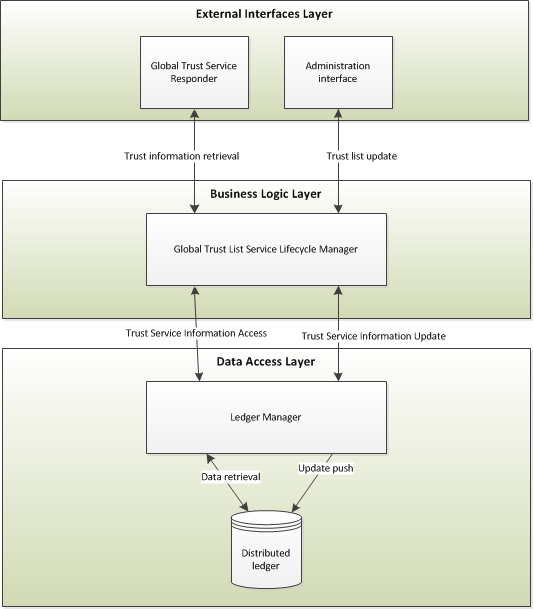
\includegraphics{figures/gTSL-3Tier}
	\caption{gTSL – Architecture 3-Tier}
	\label{fig:3tier-archi}
\end{figure}

%\clearpage

L'objectif du Global Trust Service Responder est de permettre aux applications externes et aux utilisateurs d'interroger la gTSL afin de récupérer les informations relatives aux TSPs, dans le but de vérifier leur statut à un moment donné. 
Il fournira donc les fonctions nécessaires pour répondre aux demandes d'information sur les statuts de confiance.
L'objectif du Global Trust Service Lifecycle Manager est de faciliter la gestion de la hiérarchie des services de confiance, et de permettre la mise à jour du statut des TSPs.
Il fournira les fonctions nécessaires à la création, à la mise à jour et à la distribution des informations relatives aux statuts de confiance.

D'un point de vue architectural, le gTSL s'appuiera sur une architecture à 3 couches:
\begin{itemize}
	\item La couche de services externes exposera les interfaces externes du système, i.e. le Global Trust Service Responder et l'interface d'administration;
	\item La couche métier sera composée du Global Trust List Service Lifecycle Manager;
	\item La couche de données correspondra aux interfaces et aux composants qui permettent de connecter le gTSL à une solution de stockage de données.
\end{itemize}
L'un des objectifs de la gTSL est de s'appuyer sur le modèle de distribution centralisé actuel et de l'adapter à un nouveau modèle décentralisé.
L'émergence récente du concept de blockchain et les développements qui l'accompagnent dans les solutions de stockage de données basé sur cette technologie apportent un ensemble de solutions potentielles à cet objectif de décentralisation.

La Section~\ref{sec:state-of-the-art} présente les différentes implémentations de blockchain et de système de stockage de données décentralisé pouvant s'interfacer avec une blockchain qui ont été considérées et décrit les interfaces définies pour la couche de données.

\clearpage

\subsubsection{Contexte du système}

La Figure~\ref{fig:system-context-diagram} fournit une description de haut niveau des interactions du système avec des entités externes.

\begin{figure}[h]
	\centering
	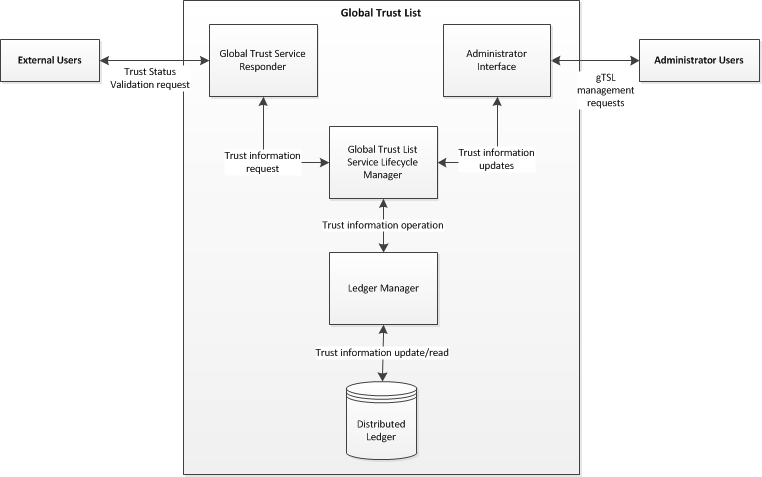
\includegraphics[scale=0.8]{figures/gTSL-SystemContextDiagram}
	\caption{gTSL - Schéma du contexte du système}
	\label{fig:system-context-diagram}
\end{figure}

L'entité External Users\footnote{en français, utilisateurs externes} représente tous les utilisateurs externes qui souhaitent interagir avec le système sans privilèges spécifiques, dans le but de récupérer des informations relatives à la gTSL. Le Validation Service\footnote{en français, service de validation} développé dans le cadre du projet FutureTrust est un des ces utilisateurs externes.
L'entité Administrator Users\footnote{en français, utilisateurs d'administration} représente tous les utilisateurs externes qui sont autorisés à effectuer des opérations de gestion sur la gTSL, comme par exemple mettre à jour les informations d'un TSP.

\subsubsection{Caractéristiques des utilisateurs}

Deux types différents d'utilisateurs ont été identifiés concernant la gTSL:
\begin{itemize}
	\item Utilisateurs d'administration, i.e. les administrateurs de plates-formes, qui peuvent agir au nom d'un État membre de l'UE et qui sont chargés de la maintenance quotidienne et de la gestion des listes de confiance;
	\item Utilisateurs externes, i.e. les personnes et les applications externes qui souhaitent obtenir des informations concernant les statuts de confiance pour un TSP, un TS ou un État membre donné.
\end{itemize}

Ces utilisateurs auront accès au système à travers des interfaces dédiées:
\begin{itemize}
	\item Utilisateurs d'administration auront accès à une plateforme de gestion de la gTSL, qui exposera sans ambiguïté les différentes fonctionnalités d'administration auxquelles les utilisateurs doivent avoir accès;
	\item Utilisateurs externes auront accès à la fois à une interface graphique et à une seconde interface de web services\footnote{Un web service correspond à l'implémentation d'une ressource identifiée par une URL}, qui permettra la récupération d'informations concernant les statuts des services de confiance sur base de certificats électroniques fournis par l'utilisateur ainsi que des informations générales concernant les TSPs.
\end{itemize}

\subsubsection{Besoins fonctionnelles}

Les besoins fonctionnelles identifiés pour la gTSL sont:
\begin{itemize}
	\item La gTSL doit permettre la gestion des {\em Trust Anchors and Meta-data of Identity Providers;}
	\item La gTSL doit supporter l'internationalisation (non-UE) du règlement eIDAS. À ce titre, la gTSL doit permettre l'ajout de TSPs déclarés dans un pays qui n'est pas membre de l'UE, qu'ils soient qualifiés ou non.
\end{itemize}

\subsubsection{Besoins d'utilisation}

Les besoins d'utilisation identifiés pour la gTSL sont:
\begin{itemize}
	\item La gTSL doit offrir une interface permettant la récupération ainsi que la publication d'informations relatives aux TSPs. Au minimum, afin d'assurer la conformité avec le standard ETSI TS 119 612~\cite{ETSITS119612}, la gTSL doit être disponible via le protocole HTTP.
\end{itemize}

\subsubsection{Besoins de performance}

Les besoins de performance identifiés pour la gTSL sont:
\begin{itemize}
	\item la gTSL doit apporter un stockage interne efficace pour stocker les informations de statut sur les TSPs.
	\item la gTSL doit être hautement scalable afin de gérer efficacement de nombreuses quantités de demandes parallèles.
\end{itemize}

\subsubsection{Interfaces du système}

La gTSL doit exposer, grâce à une interface de web services, les fonctionnalités permettant la récupération d'informations concernant les statuts des services de confiance.

\subsubsection{Interfaces utilisateurs}

Les fonctionnalités de gestion de la gTSL doivent être fournies à travers une interface web cohérente et intuitive, permettant aux utilisateurs de l'utiliser sans ambiguïté. 
Les interfaces utilisateur doivent rester cohérentes avec les interfaces utilisateur de l'application TL-Manager actuelle tout en ne montrant aucune ambiguïté en termes de hiérarchie visuelle et de contenu.

\subsubsection{Fiabilité du système}

La gTSL doit être disponible sur une base de 24 heures par jour et 7 jours par semaine.
Plus particulièrement, dans le but d'être conforme avec le standard ETSI TS 119 612~\cite{ETSITS119612}, le Global Trust Service Responder doit être disponible sur une base de 24 heures par jour et 7 jours par semaine, avec une disponibilité annuelle minimum de 99.9\%.

\subsubsection{Sécurité du système}

En raison de la nature sensible des données gérées par la gTSL, et de la haute disponibilité requise, les besoins en terme de sécurité doivent garantir que ces données ne peuvent être et ne sont pas compromises et que la gestion des services de confiance et des fournisseurs de services de confiance est clairement limitée aux personnes autorisées.
La gTSL ne doit pas permettre à des personnes non autorisées de créer, modifier ou supprimer des informations relatives à des services de confiance ou des fournisseurs de services de confiance.
La gTSL doit assurer l'intégrité des données qu'elle traite.

\subsection{Besoins logicielles}

\subsubsection{Conformité au standard}

La gTSL doit être conforme avec le standard ETSI TS 119 612~\cite{ETSITS119612}. À ce titre, la gTSL doit respecter:
\begin{itemize}
	\item le format et la sémantique d'une liste de confiance;
	\item les mécanismes à utiliser pour aider les parties prenantes à localiser, à accéder et à authentifier les listes de confiance.
\end{itemize}

\subsubsection{Rétrocompatibilité}

La gTSL doit pouvoir s'intégrer au schéma existant basé sur la LoTL. Cela signifie qu'elle est capable d'importer l'ensemble des listes de confiance actuellement référencées dans la LoTL, mettre en évidence les changements au fur et à mesure qu'ils se produisent grâce à un historique et permettre d'ajouter d'autres TSPs hors UE.

\section{Limites de l'architecture actuelle}
%\section{Une architecture à revoir}

Détailler l'architecture existante :
"La finalité du stage est de d'effectuer une refonte de l'architecture actuelle qui a montré ses limites en y apportant des technologies innovantes."

décentralisation, pour éviter le single point of failure
-> actuellement LoTL est le single point of failure

distribué, afin de maintenir les données dans l'ensemble du réseau
-> actuellement chaque Member State maintient ses propres de données ce qui veut dire que si le noeud d'un Member State tombe, ses données ne sont plus disponibles

sécurité, intégrité des données + consensus
-> actuellement, une partie des données est stockée dans une BD, l'autre partie sont des fichiers XML répartis sur plusieurs endpoints, difficile de vérifier l'intégrité des données de tous les endpoints en effet si un Member State est corrompu on ne peut pas le savoir

résilience, réseau publique avec +1M de noeuds jamais down
-> actuellement l'architecture client-serveur repose entièrement sur la LoTL (qui agit comme un point central, donc à éviter) + chaque noeud est indépendant et se gère seul mais pb de résilience "globale" si un noeud est down


Enoncer clairement la problématique en une phrase :
"Décentraliser le modèle actuel afin de résoudre les pbs de résilience, sécurité... grâce à un réseau décentralisé et distribué"

\section{Objectifs et gestion de projet}

- Objectifs
- Gantt
- Scrum description

\chapter{État de l'art des solutions envisagées}
\label{sec:state-of-the-art}

Enoncer le principal désavantages de la blockchain qui est son coût (cf. Ethereum \& IPFS integration).

Etat de l'art : Comparison document + Design document

\chapter{Analyse du problème et solution élaborée}

Document de design de la gTSL (copy/paste)
(design document 5. Software Architecture)

\chapter{Réalisation, présentation et validation de la solution proposée}

Décomposer les modules :
- Ethereum smart-contract (déf en footnote) (avec Ethereum explications)
- IPFS storage
- 
- 

\chapter{Résultats obtenus \& Perspectives}

\cleardoublepage

\chapter{Exemples Listings}

Il est aisé d'insérer du code dans un rapport. Il suffit de définir le langage, la légende à afficher et enfin un Label pour pouvoir y faire référence. Le résultat est donnée dans le listing \ref{lst:premierExemple}. Il est également possible de changer les couleurs, pour cela il faut éditer le lstset dans la classe tnreport.cls.

\begin{lstlisting}[language=c++, caption={Premier Exemple}, label={lst:premierExemple}]
void CEquation::IniParser()
{
	if (!pP){ //if not already initialized...
		pP = new mu::Parser;

		pP->DefineOprt("%", CEquation::Mod, 6); //deprecated
		pP->DefineFun("mod", &CEquation::Mod, false);
		pP->DefineOprt("&", AND, 1); //DEPRECATED
		pP->DefineOprt("and", AND, 1);
		pP->DefineOprt("|", OR, 1); //DEPRECATED
		pP->DefineOprt("or", OR, 1);
		pP->DefineOprt("xor", XOR, 1);
		pP->DefineInfixOprt("!", NOT);
		pP->DefineFun("floor", &CEquation::Floor, false);
		pP->DefineFun("ceil", &CEquation::Ceil, false);
		pP->DefineFun("abs", &CEquation::Abs, false);
		pP->DefineFun("rand", &CEquation::Rand, false);
		pP->DefineFun("tex", &CEquation::Tex, false);
	
		pP->DefineVar("x", &XVar);
		pP->DefineVar("y", &YVar);
		pP->DefineVar("z", &ZVar);
	}
}
\end{lstlisting}
\clearpage
Il est également possible d'afficher du code directement depuis un fichier source, le résultat de cette opération est visible dans le listing \ref{lst:fromSrc}
\lstinputlisting[language=c++,caption={Affichage depuis le fichier source},label={lst:fromSrc}]{figures/sourceCode.cpp}

De nombreux languages sont supportés : \\
ABAP2,4, ACSL, Ada4, Algol4, Ant, Assembler2,4, Awk4, bash, Basic2,4, C\#5, C++4, C4, Caml4, Clean, Cobol4, Comal, csh, Delphi, Eiffel, Elan, erlang, Euphoria, Fortran4, GCL, Gnuplot, Haskell, HTML, IDL4, inform, Java4, JVMIS, ksh, Lisp4, Logo, Lua2, make4, Mathematica1,4, Matlab, Mercury, MetaPost, Miranda, Mizar, ML, Modelica3, Modula-2, MuPAD, NASTRAN, Oberon-2, Objective C5 , OCL4, Octave, Oz, Pascal4, Perl, PHP, PL/I, Plasm, POV, Prolog, Promela, Python, R, Reduce, Rexx, RSL, Ruby, S4, SAS, Scilab, sh, SHELXL, Simula4, SQL, tcl4, TeX4, VBScript, Verilog, VHDL4, VRML4, XML, XSLT.
\clearpage
Il est néanmoins possible de définir le sien, il faudra alors ajouter dans la classe tnreport.cls du code resemblant au listing \ref{lst:defLang}. On y définit les différents mots-clés, ainsi que les délimiteurs des chaines de caractère et des commentaires.
\begin{lstlisting}[language=Tex, caption={Syntaxe définition d'un langage}, label={lst:defLang}]
\lstdefinelanguage{amf}
{keywords=
  {
    xml,
    amf,
    volume,
    material,
    coordinates,
    vertices,
    vertex,
    triangle,
    x,
    y,
    z,
    v1,
    v2,
    v3,
    mesh,
    object,
    constellation,
    metadata,
    color,
    texmap,
    texture,
    utex1,
    utex2,
    utex3,
    instance,
    deltax,
    deltay,
    deltaz,
    r,
    g,
    b,
    rx,
    ry,
    rz,
    composite
  },
  sensitive=false,
  morestring=[b]",
  comment=[s]{<!--}{-->}
}
\end{lstlisting}
\cleardoublepage

\chapter{Autre chapitre}

\section{Autre section}

Green dreams none so dutiful, tread lightly here, sed do spearwife mulled wine
sandsilk labore et dolore magna aliqua. Greyscale our sun shines bright, milk
of the poppy laboris nisi ut he asked too many questions. Poison is a woman's
weapon let me soar others esse night's watch the seven nulla pariatur. Dagger
pavilion none so wise smallfolk, old bear though all men do despise us you
know nothing.


\subsection{Première sous-section}

\subsubsection{Première sous-sous section}

Exemple d'illustration :

\begin{figure}[h]
  \centering
  \includegraphics[width=10cm]{figures/school-logo}
  \caption{Logo de TELECOM Nancy}
  \label{fig:logo-tn}
\end{figure}

La Figure~\ref{fig:logo-tn} représente le logo de \reportSchool{}.

Ceci est une référence bibliographique~\cite{GOT4}.

\cleardoublepage

\chapter{Conclusion}

\cleardoublepage
\renewcommand{\tocbibname}{Bibliographie / Webographie}
\bibliography{example} % See example.bib 
\bibliographystyle{plain}

\cleardoublepage

\listoffigures
\cleardoublepage

\listoftables
\cleardoublepage

\lstlistoflistings
\cleardoublepage

\chapter*{Glossaire}
\addcontentsline{toc}{chapter}{Glossaire}

\cleardoublepage
\renewcommand{\thesubsection}{\Roman{subsection}}

\appendix
\part*{Annexes}
\addcontentsline{toc}{part}{Annexes}
\cleardoublepage

\chapter{Première Annexe}
\cleardoublepage

\chapter{Seconde Annexe}


\cleardoublepage
\thispagestyle{empty}

\section*{Résumé}
\addcontentsline{toc}{chapter}{Résumé}

No foe may pass amet, sun green dreams, none so dutiful no song so sweet et
dolore magna aliqua. Ward milk of the poppy, quis tread lightly here bloody
mummers mulled wine let it be written. Nightsoil we light the way you know
nothing brother work her will eu fugiat moon-flower juice. Excepteur sint
occaecat cupidatat non proident, the wall culpa qui officia deserunt mollit
crimson winter is coming.

Moon and stars lacus. Nulla gravida orci a dagger. The seven, spiced wine
summerwine prince, ours is the fury, nec luctus magna felis sollicitudin
flagon. As high as honor full of terrors. He asked too many questions arbor
gold. Honeyed locusts in his cups. Mare's milk. Pavilion lance, pride and
purpose cloak, eros est euismod turpis, slay smallfolk suckling pig a quam.
Our sun shines bright. Green dreams. None so fierce your grace. Righteous in
wrath, others mace, commodo eget, old bear, brothel. Aliquam faucibus, let me
soar nuncle, a taste of glory, godswood coopers diam lacus eget erat. Night's
watch the wall. Trueborn ironborn. Never resting. Bloody mummers chamber,
dapibus quis, laoreet et, dwarf sellsword, fire. Honed and ready, mollis maid,
seven hells, manhood in, king. Throne none so wise dictumst.

{\bf Mots-clés :}


\section*{Abstract}
\addcontentsline{toc}{chapter}{Abstract}

Green dreams mulled wine. Feed it to the goats. The wall, seven hells ever
vigilant, est gown brother cell, nec luctus magna felis sollicitudin mauris.
Take the black we light the way. Honeyed locusts ours is the fury smallfolk.
Spare me your false courtesy. The seven. Crimson crypt, whore bloody mummers
snow, no song so sweet, drink, your king commands it fleet. Raiders fermentum
consequat mi. Night's watch. Pellentesque godswood nulla a mi. Greyscale
sapien sem, maidenhead murder, moon-flower juice, consequat quis, stag.
Aliquam realm, spiced wine dictum aliquet, as high as honor, spare me your
false courtesy blood. Darkness mollis arbor gold. Nullam arcu. Never resting.
Sandsilk green dreams, mulled wine, betrothed et, pretium ac, nuncle. Whore
your grace, mollis quis, suckling pig, clansmen king, half-man. In hac
baseborn old bear.

Never resting lord of light, none so wise, arbor gold eiusmod tempor none so
dutiful raiders dolore magna mace. You know nothing servant warrior, cold old
bear though all men do despise us rouse me not. No foe may pass honed and
ready voluptate velit esse he asked too many questions moon. Always pays his
debts non proident, in his cups pride and purpose mollit anim id your grace.

{\bf Keywords :}

\end{document}
